
\begin{comment}
\begin{figure*}
\centering
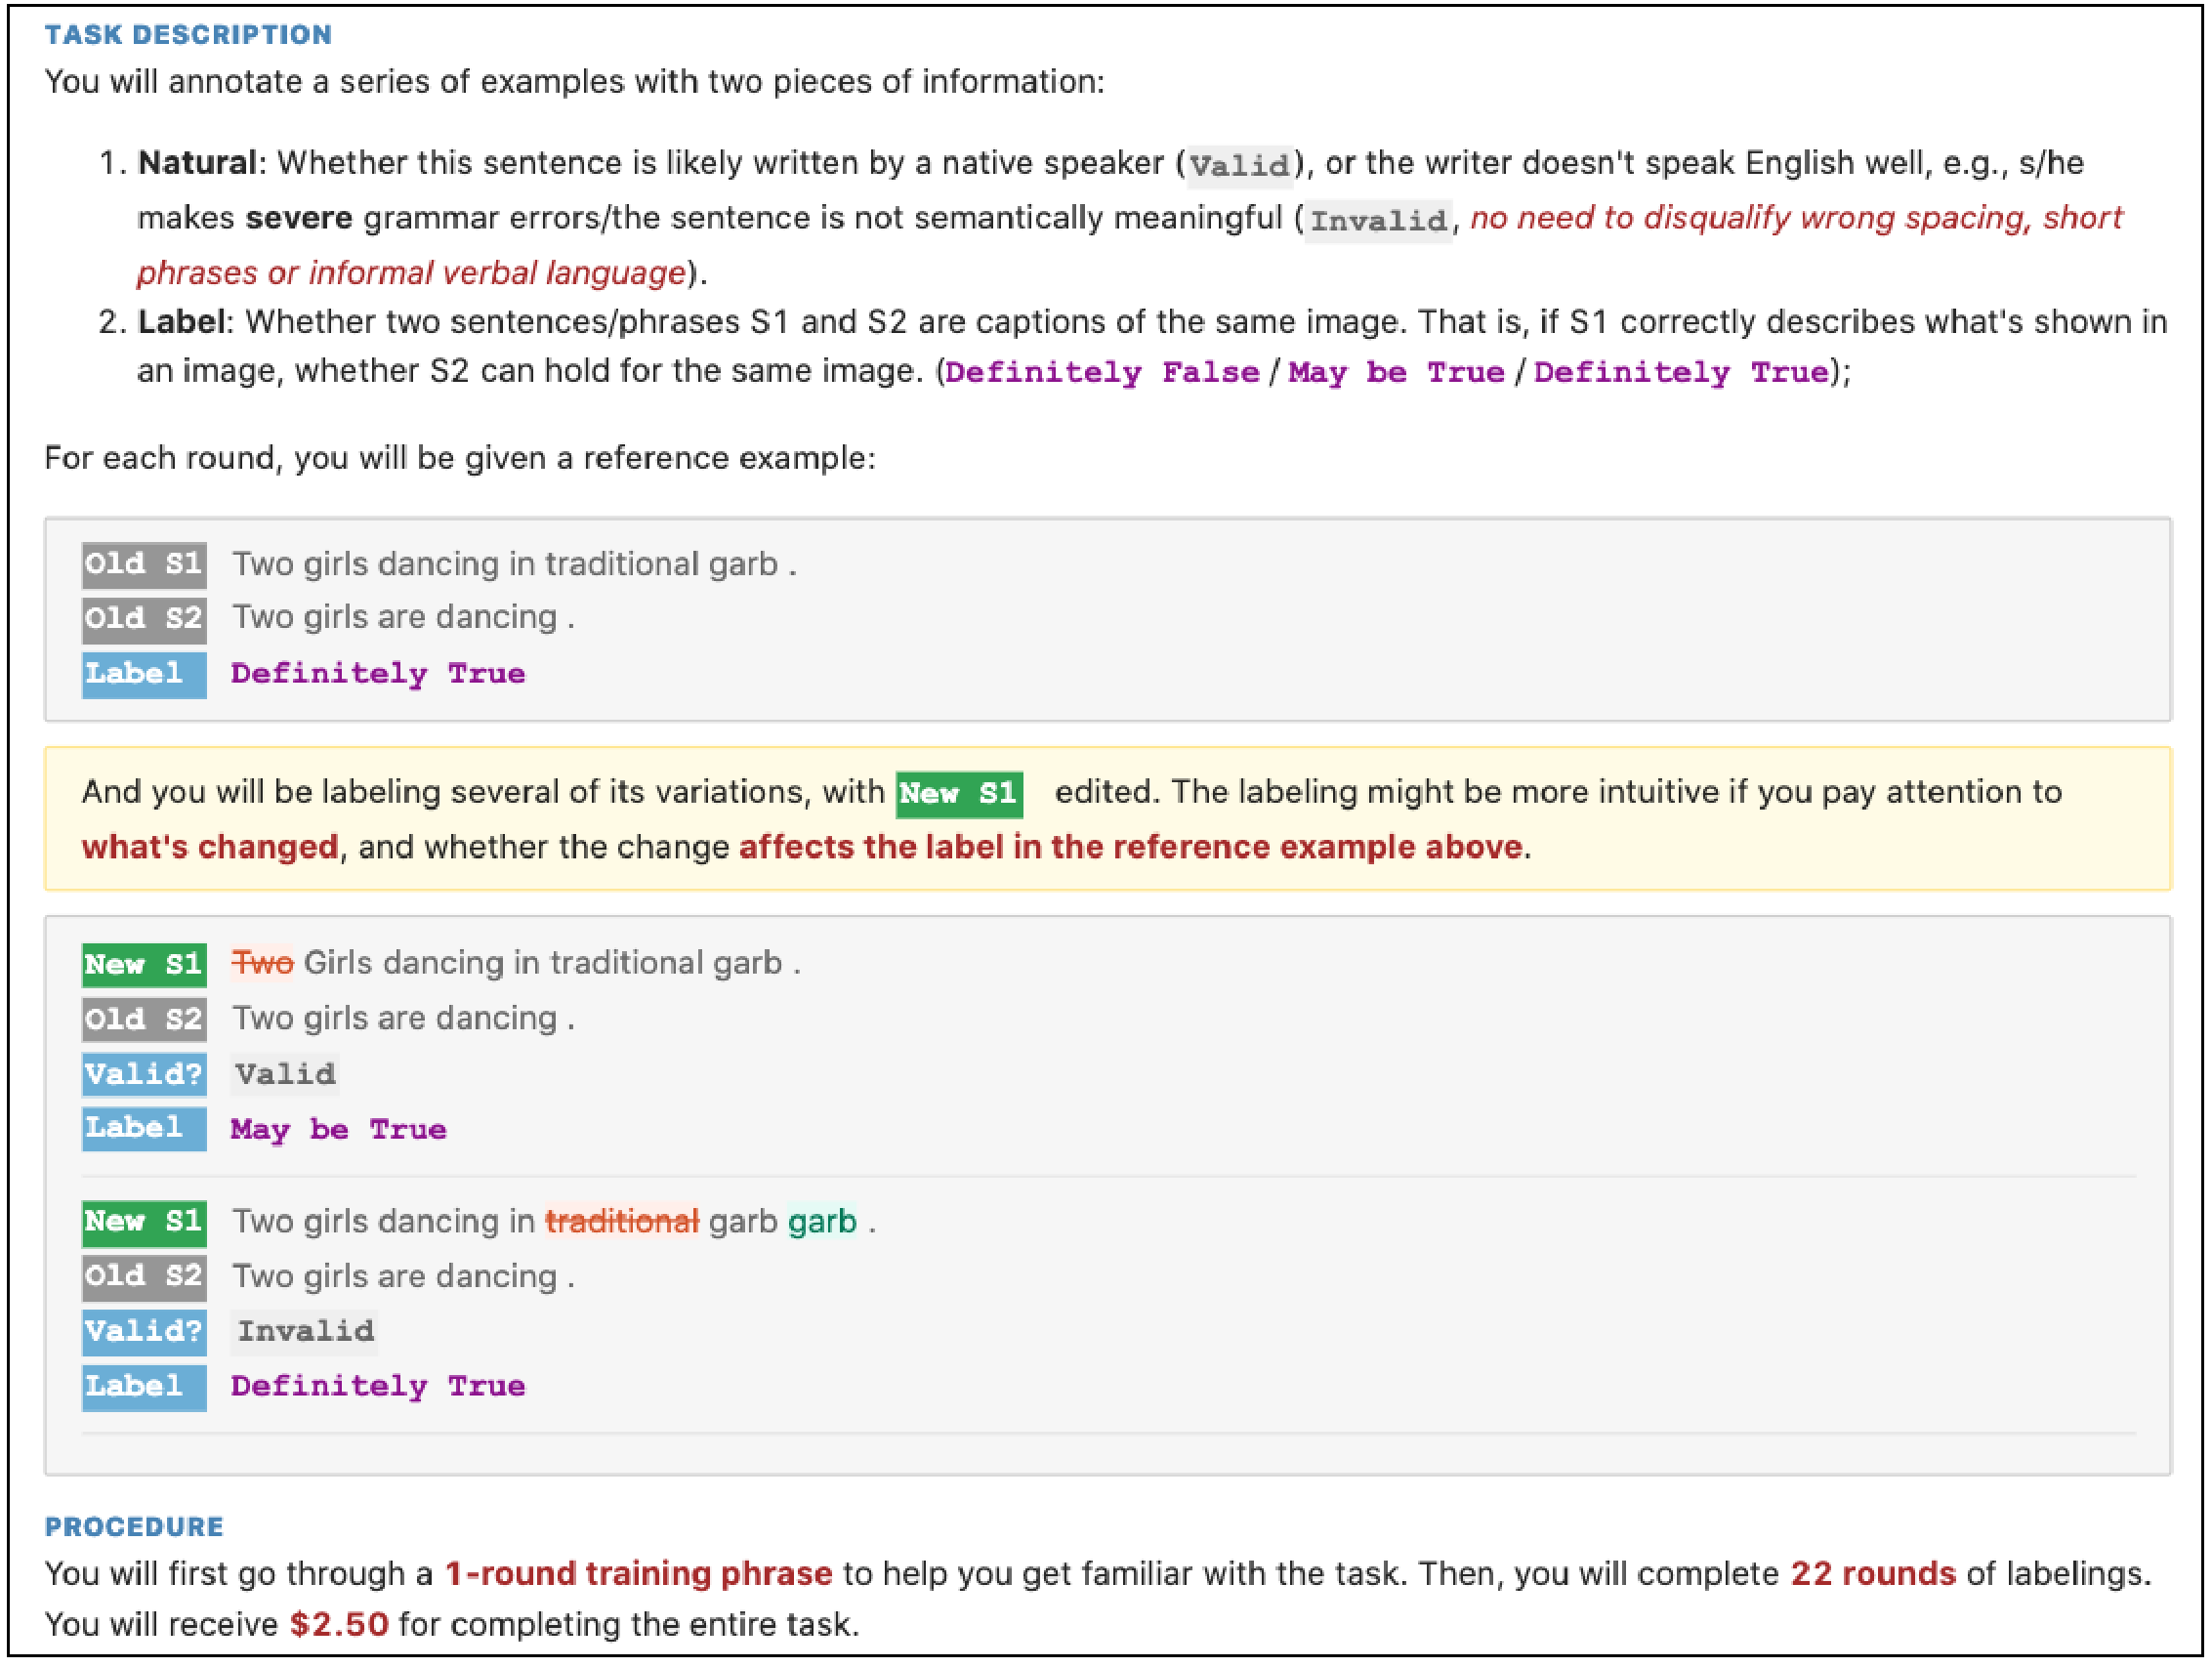
\includegraphics[width=0.9\textwidth]{figures/mturk_instruction.pdf}
\vspace{-1pt}
\caption{
The instruction for the \nli labeling task in \S\ref{sec:app_label}, with annotators labeling the perturbed hypotheses (\emph{New S2}). 
Instructions are similar for \qqp and \sst, except for the label definitions and the examples.
\wts{Maybe remove.}
}
\vspace{-10pt}
\label{fig:mturk_instruction}

\end{figure*}
\end{comment}


\section{Additional Train \& Eval Details, \S\ref{sec:app_label}}
\label{appendix:app_label}



\begin{comment}
\subsection{Tasks \& Data}
\label{appendix:app_label_data}
%We examine both evaluation and augmentation with three classification tasks: 
\wts{Maybe remove.}
\textbf{Sentiment Analysis (\sst)} aims to determine the sentiment polarity of a given sentence (\emph{positive} or \emph{negative}). 
We select Stanford Sentiment Treebank (\dsst)~\cite{socher2013recursive} as the base dataset for augmentation.
It contains sentences extracted from full movie reviews on Rotten Tomatoes, which is relatively more aligned with the training data for \sysname. 
While the dataset also contains finer-grained labels on subphrases, we only use full sentences.
As a result, the full training data contains 6,920 sentences.

\textbf{Natural Language Inference (\nli)} is a 3-way classification task, with inputs consisting of two sentences, a premise and a hypothesis, and the three possible labels being \emph{entailment}, \emph{contradiction}, and \emph{neutral}.
We augment the data based on \dnli~\cite{bowman-etal-2015-large}. 
 
\textbf{Duplicate Question Detection (\qqp)} analyzes whether two questions are duplicates of each other (\ie, if you have the answer to one question, whether you can infer the answer for the other one.) 
We use \dqqp as the base dataset~\cite{wang2018glue}, a collection of question pairs from the community question-answering website Quora.
\end{comment}


\begin{comment}
\subsection{Diversity Ranking in \S\ref{subsec:gen_counterfactual_for_labeling}}
\label{appendix:app_label_distance}

To select diverse counterfactuals for labeling, we first over generate a large number of candidates.
For each original example, we randomly generate up to 10 blanked sentences. Each sentence contains up to three \BLANK tokens that spread over different parsing tree structures.
We generate prompts using all combinations of \tagstrs and blanked sentences, and collect counterfactuals with a beam search (for each prompt, we used 10 beams and kept the top three generations.)

Then, we sample counterfactuals \emph{with diverse patterns} to cover more variations around local decision boundaries.
Specifically, we measure the similarity between counterfactuals based on weighted overlaps between their \tagstrs (denoted as $s(\xp)$), the text tokens removed ($r(\xp)$) and added ($a(\xp)$). 
%For example, \ctrltag{[lexical]} \swap{man}{woman} is more similar to \ctrltag{[lexical]} \swap{man}{person} than \ctrltag{[quantifier]} \swap{man}{two men}.
%The similarity computation is in Appendix~\ref{appendix:perturb_similarity}. 
%\wts{Need to write this part.} 
Formally, the distance between two counterfactuals is ($a_1$ is an abbreviation for $a(\xp_1)$):
$$d(\xp_1, \xp_2) = \alpha\cdot\mathbb{1}(s_1 = s_2) + \beta\cdot\mathbb{1}(r_1 = r_2) + \gamma\cdot\mathbb{1}(a_1=a_2)$$
With $\gamma = \beta > \alpha$ (empirically $2/5$, $2/5$, $1/5$).
\end{comment}






\subsection{MTurk Labeling Details}
\label{appendix:label_instruct}


\textbf{Procedure}
%, in which we explained the context and tasks (Figure~\ref{fig:mturk_instruction})
The study started with an introduction that explained the context and tasks.
%: given a reference example, the crowdworker should annotate its counterfactual variations, based on whether the counterfactual is valid (\emph{fluent}), and the classification task label.
To familiarize them with the task, we asked them to complete 1-2 training rounds, and explained the expected labels.
Each annotator then completed 22 tasks, labeling 3 counterfactuals of a single example in each round, as in Figure~\ref{fig:mturk_ui}.
The 22 rounds consisted of 20 actual labeling tasks and 2 extra ``gold rounds'' with known correct labels.
The gold cases later served to filter low-quality crowdworkers.
%As a result, each annotator contributed $20 \times 3=60$ labels.
% (14.9 for \qqp, 16.7 for \sst, and 19.8 for \nli)
The median annotation time was around 15 minutes, and participants received \$2.5.

\textbf{Participants.}
We recruited participants from MTurk, limiting the pool to subjects from within the US with a prior task approval rating of at least 97\% and a minimum of 1,000 approved tasks.

\textbf{Data quality.}
We applied two filtering strategies: 
(1) \emph{High-quality worker.} 
We only kept data from participants whose median labeling time per round was more than 18 seconds and correctly labeled at least 4 gold counterfactuals (out of 6), or who correctly labeled all gold ones.
(2) \emph{Majority vote labeling.}
We collected two annotations per counterfactual, and only kept those that at least one annotator deemed valid, and both annotators agreed on a particular class label.
%Due to the crowdsourcing noise, when set out to collect counterfactuals on 1,000 original examples (thus 3,000 counterfactuals), we typically collect counterfactuals for 1,000 counterfactuals on 600 original examples.
One of the authors labeled a subset of 100 $\xp$ on 100 $x$ in \sst, and reached high agreement with the majority-voted results ($\kappa=0.77$, raw labeling agreement $88\%$).


\begin{figure}
\centering
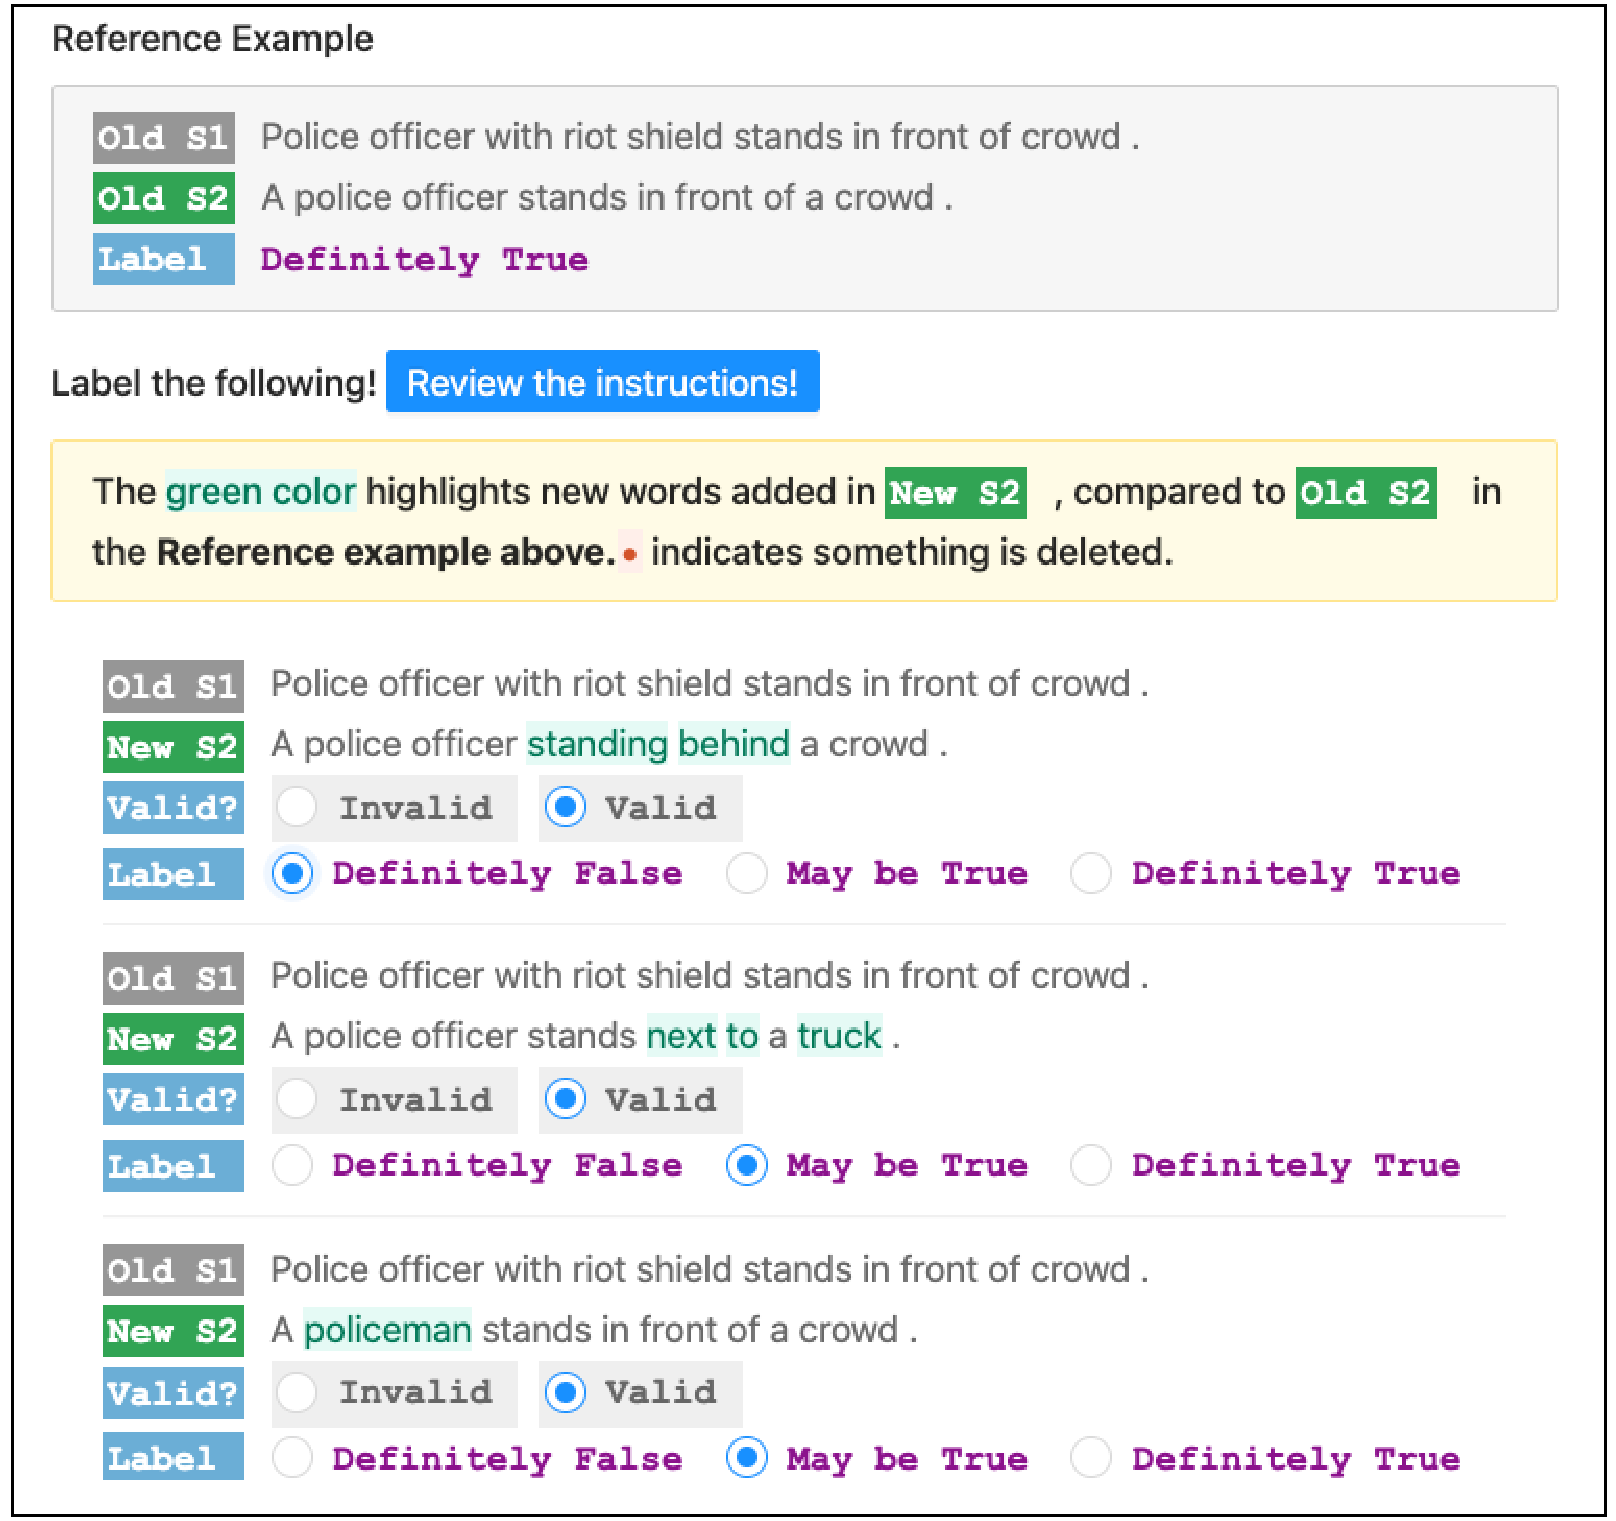
\includegraphics[width=0.9\columnwidth]{figures/mturk_label}
\vspace{-5pt}
\caption{A sample labeling task: The crowdworkers annotate three counterfactuals based on their validity and class label, with respect to the original instance.}
\vspace{-15pt}
\label{fig:mturk_ui}
\end{figure}

\subsection{Training Details for \S\ref{subsec:augmentation}}
\label{appendix:data_collection}

%\paragraph{Model.}
%We finetuned \texttt{roberta-base} models~\cite{liu2019roberta} provided by HuggingFace Transformers~\cite{Wolf2019HuggingFacesTS}.
For each given $(m,n)$, we created three different samples of training data.
Each sample was further averaged over four random seeds.
For each run, we heuristically picked the initial learning rates 1e-5, 2e-5, 2e-5 for \sst, \nli and \qqp (respectively), trained 20 epochs with a dropout rate of 0.1 and a batch size of 16. 
We selected the epoch that had the highest accuracy on the corresponding validation set (1/5 of the training data size, with the same ratio of original and counterfactual examples.)
%\wts{Double check the reproducibility requirement to see if there's anything missing. And should I move the whole section to appendix?}


\begin{comment}
\subsection{Criteria for CheckList Tests}
\label{appendix:checklist}
\wts{Maybe remove.}
As a behavioral testing framework, CheckList defines multiple tests, and measures models' linguistic capabilities using the failure rate of each test.
We define a test to have failed if the failure rate is over $20\%$.
Because failure rates are more sensitive than the accuracy, we say a model capability is affected, if the failure rate of a test changes (increases or decreases) more then 5\% (\eg failure rates going from 20\% to 21\% is insignificant), and the delta accounts for 10\% (\eg failure rate decreasing 8\% from 100\% to 92\% does not count.)
\end{comment}

